\documentclass[a4pape]{article}
\usepackage[utf8]{inputenc}
\usepackage{tikz}
\usepackage{pdflscape}
\usetikzlibrary{mindmap}

%%%% Predefined Colors: black, blue, brown, cyan, darkgray, gray, green, lightgray, lime, magenta, olive, orange, pink, purple, red, teal, violet, white, yellow.

\pagestyle{empty}
\begin{document}

%%%%%%%%%%%%%%%%%%%%%%%%%%%%%%%%%%%%%%%% Überblick
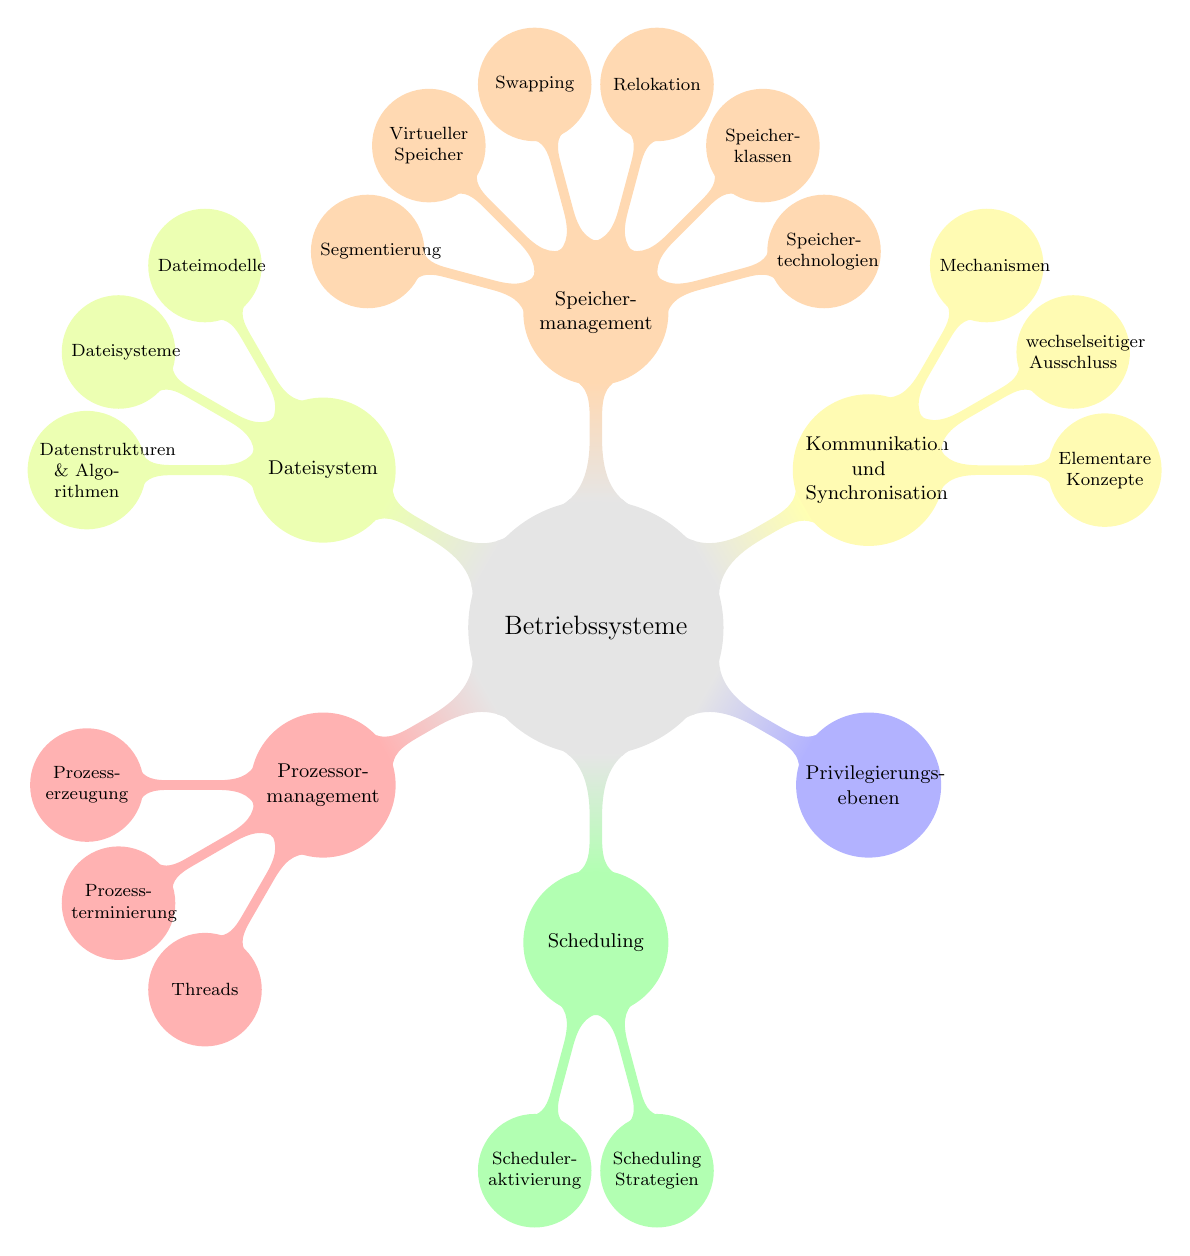
\begin{tikzpicture}[ mindmap, grow cyclic, every node/.style=concept, concept color=black!10,
    level 1/.append style={level distance=4cm},
    level 2/.append style={level distance=3cm, sibling angle=30},
    every node/.append style={scale=0.8}]

  \node{Betriebssysteme}
  child [concept color=red!30]{ node {Prozessor-management}
      child { node {Prozess-erzeugung}}
      child { node {Prozess-terminierung}}
      child { node {Threads}}
    }
  child [concept color=green!30]{ node {Scheduling}
      child { node {Scheduler-aktivierung}}
      child { node {Scheduling Strategien}}
    }
  child [concept color=blue!30]{ node {Privilegierungs-ebenen}}
  child [concept color=yellow!30]{ node {Kommunikation und\\Synchronisation}
      child { node {Elementare Konzepte}}
      child { node {wechselseitiger Ausschluss}}
      child { node {Mechanismen}}
    }
  child [concept color=orange!30]{ node {Speicher-management}
      child { node {Speicher-technologien}}
      child { node {Speicher-klassen}}
      child { node {Relokation}}
      child { node {Swapping}}
      child { node {Virtueller Speicher}}
      child { node {Segmentierung}}
    }
  child [concept color=lime!30]{ node {Dateisystem}
      child { node {Dateimodelle}}
      child { node {Dateisysteme}}
      child { node {Datenstrukturen \& Algorithmen}}
    };
\end{tikzpicture}

%%%%%%%%%%%%%%%%%%%%%%%%%%%%%%%%%%%%%% Grundbegriffe
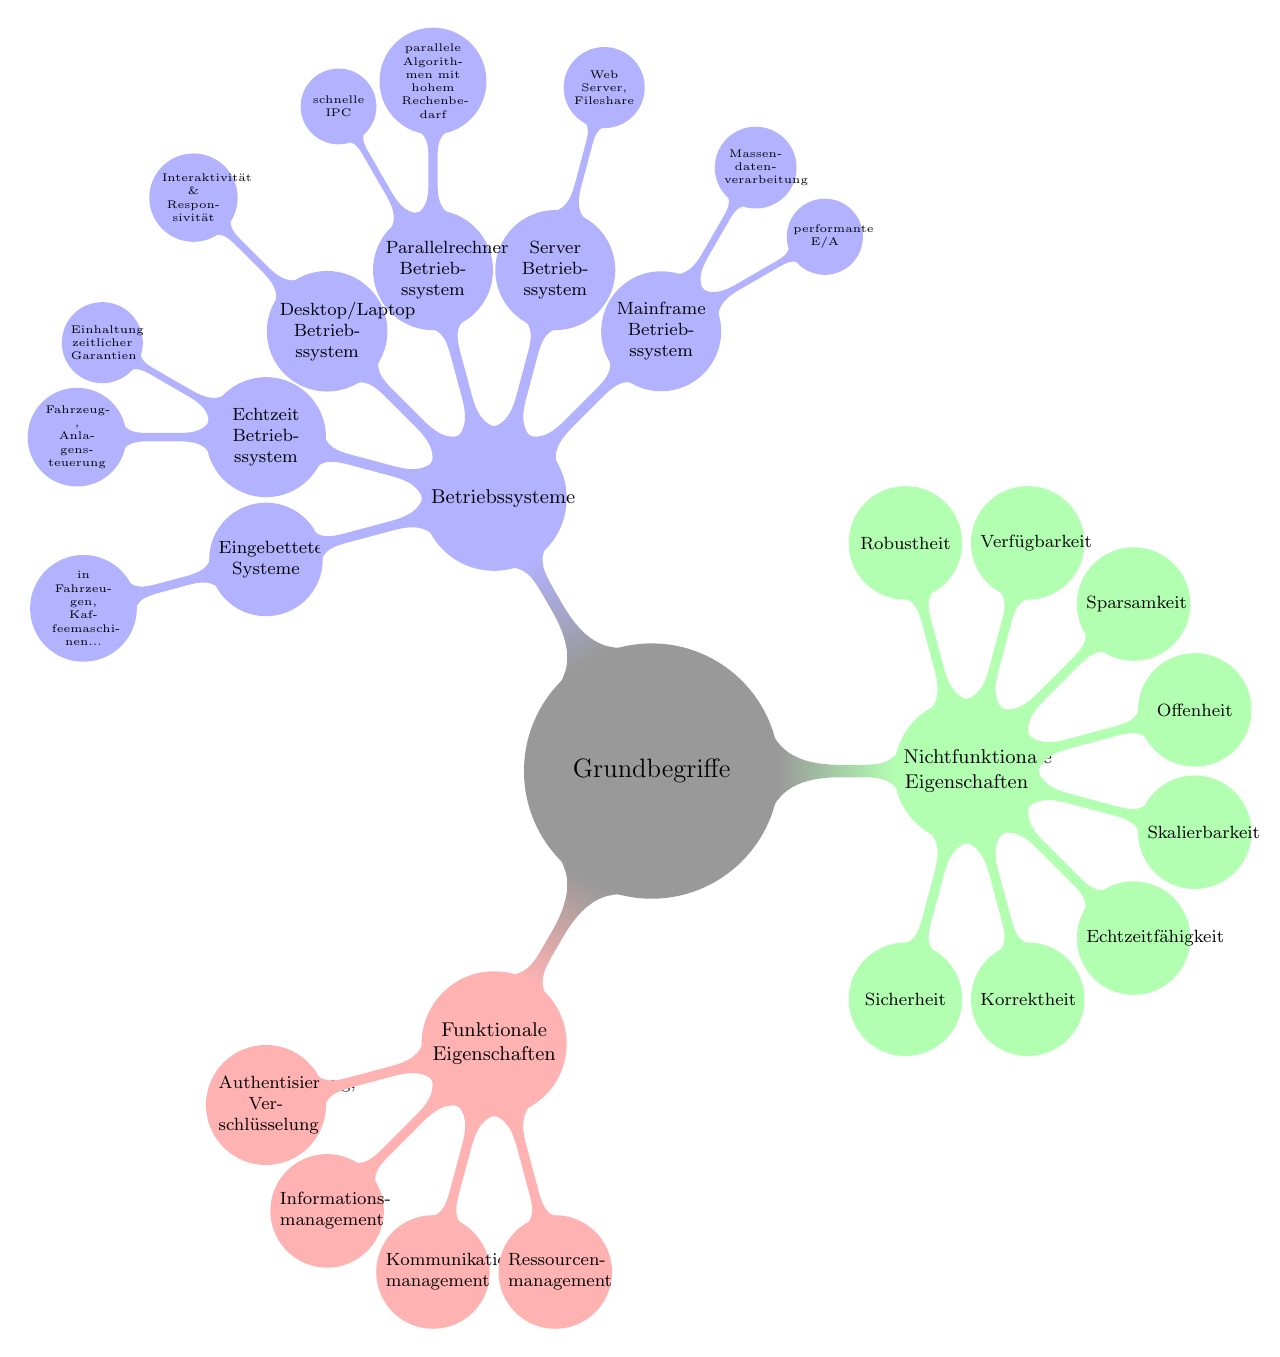
\begin{tikzpicture}[ mindmap, grow cyclic, every node/.style=concept, concept color=black!40,
    level 1/.append style={level distance=4cm, sibling angle=120},
    level 2/.append style={level distance=3cm, sibling angle=30},
    every node/.append style={scale=0.8}]
  \node{Grundbegriffe}
  child[concept color=red!30]{node{Funktionale Eigenschaften}
      child{node{Authentisierung, Verschlüsselung}}
      child{node{Informations-management}}
      child{node{Kommunikations-management}}
      child{node{Ressourcen-management}}
    }
  child[concept color=green!30]{node{Nichtfunktionale Eigenschaften}
      child{node{Sicherheit}}
      child{node{Korrektheit}}
      child{node{Echtzeitfähigkeit}}
      child{node{Skalierbarkeit}}
      child{node{Offenheit}}
      child{node{Sparsamkeit}}
      child{node{Verfügbarkeit}}
      child{node{Robustheit}}
    }
  child[concept color=blue!30]{node{Betriebssysteme}
      child{ node {Mainframe Betriebssystem}
          child{ node {performante E/A}}
          child{ node {Massen-daten-verarbeitung}}
        }
      child{ node {Server Betriebssystem}
          child{ node {Web Server, Fileshare}}
        }
      child{ node {Parallelrechner Betriebssystem}
          child{ node {parallele Algorithmen mit hohem Rechenbedarf}}
          child{ node {schnelle IPC}}
        }
      child{ node {Desktop/Laptop Betriebssystem}
          child{ node {Interaktivität \& Responsivität}}
        }
      child{ node {Echtzeit Betriebssystem}
          child{ node {Einhaltung zeitlicher Garantien}}
          child{ node {Fahrzeug-, Anlagensteuerung}}
        }
      child{ node {Eingebettete Systeme}
          child{ node {in Fahrzeugen, Kaffeemaschinen...}}
        }
    }
  ;
\end{tikzpicture}

%%%%%%%%%%%%%%%%%%%%%%%%%%%%%%%%%%%%%% Prozessormanagement
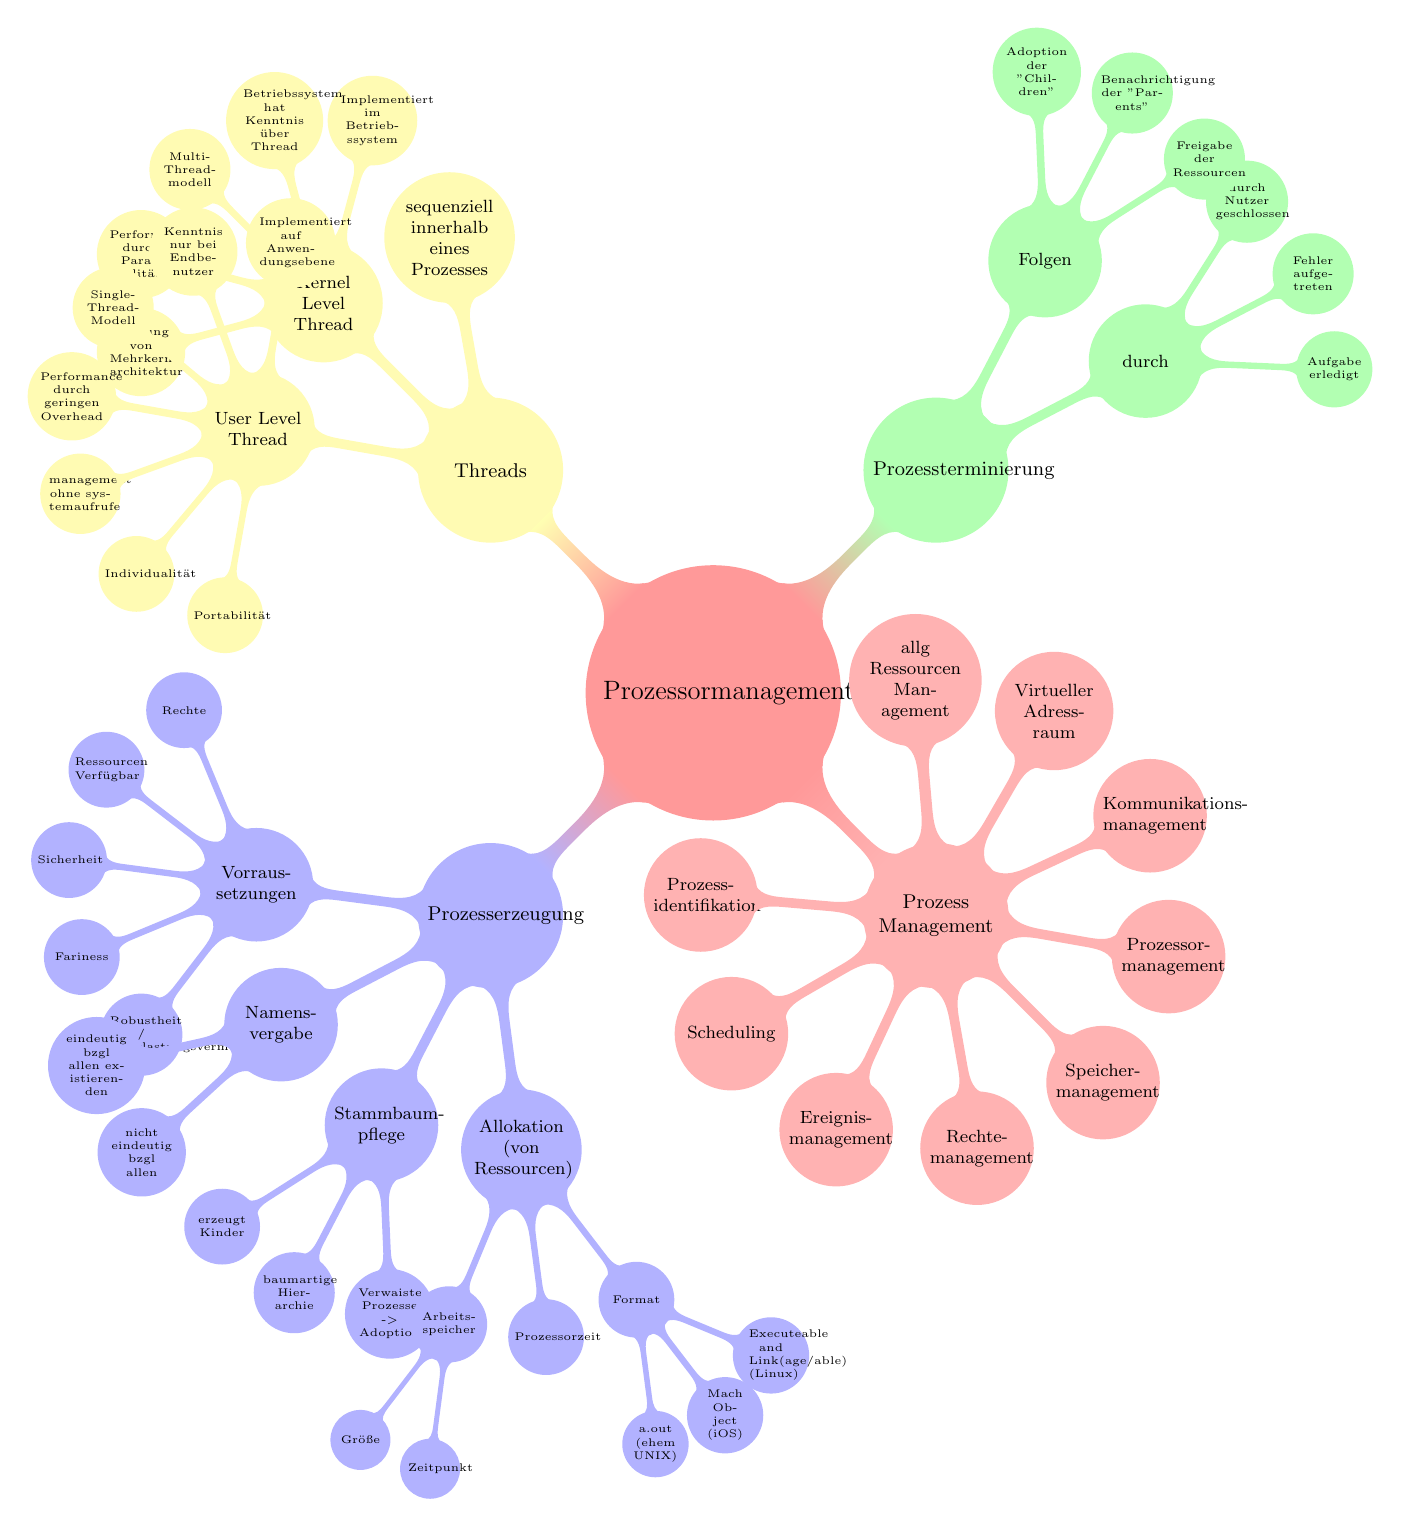
\begin{tikzpicture}[ mindmap, grow cyclic, every node/.style=concept, concept color=red!40,
    level 1/.append style={level distance=4cm, sibling angle=90},
    level 2/.append style={level distance=3cm, sibling angle=35},
    every node/.append style={scale=0.8}]
  \node{Prozessormanagement}
  child[concept color=blue!30]  { node {Prozesserzeugung}
      child { node {Vorraus-setzungen}
          child { node {Rechte}}
          child{ node {Ressourcen Verfügbar}}
          child{ node {Sicherheit}}
          child{ node{Fariness}}
          child{node{Robustheit / Überlastungsvermeidung}}
        }
      child { node {Namens-vergabe}
          child{node{eindeutig bzgl allen existierenden}}
          child{node{nicht eindeutig bzgl allen}}
        }
      child { node {Stammbaum-pflege}
          child{node{erzeugt Kinder}}
          child{node{baumartige Hierarchie}}
          child{node{Verwaiste Prozesse -> Adoption}}
        }
      child { node {Allokation (von Ressourcen)}
          child{node{Arbeits-speicher}
              child{node{Größe}}
              child{node{Zeitpunkt}}
            }
          child{node{Prozessorzeit}}
          child{node{Format}
              child{node{a.out (ehem UNIX)}}
              child{node{Mach Object (iOS)}}
              child{node{Executeable and Link(age/able) (Linux)}}
            }
        }
    }
  child[concept color=red!30]  { node {Prozess Management}
      child{node{Prozess-identifikation}}
      child{node{Scheduling}}
      child{node{Ereignis-management}}
      child{node{Rechte-management}}
      child{node{Speicher-management}}
      child{node{Prozessor-management}}
      child{node{Kommunikations-management}}
      child{node{Virtueller Adressraum}}
      child{node{allg Ressourcen Management}}
    }
  child[concept color=green!30]  { node {Prozessterminierung}
      child{node{durch}
          child{node{Aufgabe erledigt}}
          child{node{Fehler aufgetreten}}
          child{node{durch Nutzer geschlossen}}
        }
      child{node{Folgen}
          child{node{Freigabe der Ressourcen}}
          child{node{Benachrichtigung der "Parents"}}
          child{node{Adoption der "Children"}}
        }
    }
  child[concept color=yellow!30]  { node {Threads}
      child{node{sequenziell innerhalb eines Prozesses}}
      child{node{Kernel Level Thread}
          child{node{Implementiert im Betriebssystem}}
          child{node{Betriebssystem hat Kenntnis über Thread}}
          child{node{Multi-Thread-modell}}
          child{node{Performance durch Parallelität}}
          child{node{Nutzung von Mehrkern-architektur}}
        }
      child{node{User Level Thread}
          child{node{Implementiert auf Anwendungsebene}}
          child{node{Kenntnis nur bei Endbenutzer}}
          child{node{Single-Thread-Modell}}
          child{node{Performance durch geringen Overhead}}
          child{node{management ohne systemaufrufe}}
          child{node{Individualität}}
          child{node{Portabilität}}
        }
    }
  ;
\end{tikzpicture}

%%%%%%%%%%%%%%%%%%%%%%%%%%%%%%%%%%%%%% Scheduling
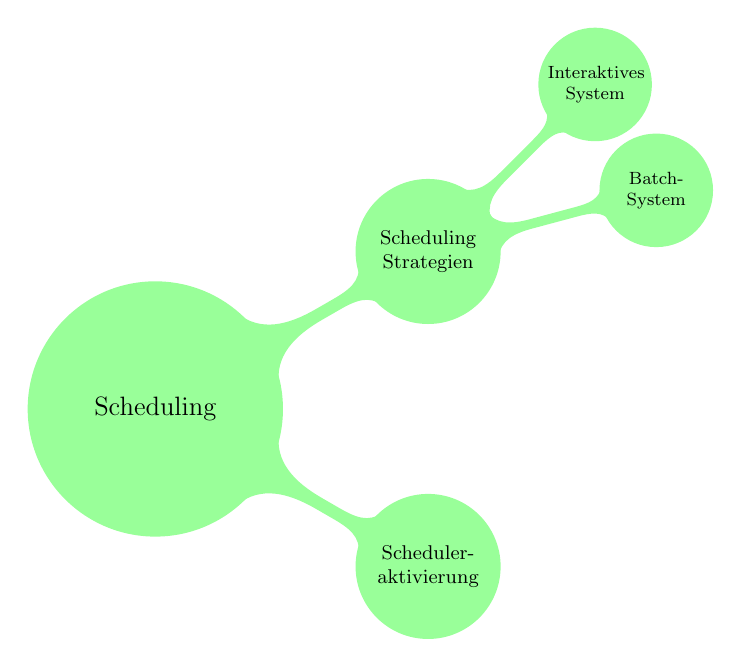
\begin{tikzpicture}[ mindmap, grow cyclic, every node/.style=concept, concept color=green!40,
    level 1/.append style={level distance=4cm},
    level 2/.append style={level distance=3cm, sibling angle=30},
    every node/.append style={scale=0.8}]
  \node{Scheduling}
  child { node {Scheduler-aktivierung}}
  child { node {Scheduling Strategien}
      child { node {Batch-System}}
      child { node {Interaktives System}}
    };
\end{tikzpicture}

%%%%%%%%%%%%%%%%%%%%%%%%%%%%%%%%%%%%%% Privilegierungsebenen
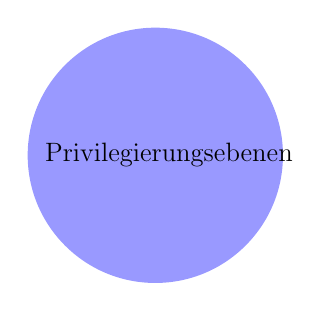
\begin{tikzpicture}[ mindmap, grow cyclic, every node/.style=concept, concept color=blue!40,
    level 1/.append style={level distance=4cm},
    level 2/.append style={level distance=3cm, sibling angle=30},
    every node/.append style={scale=0.8}]
  \node{Privilegierungsebenen};
\end{tikzpicture}

%%%%%%%%%%%%%%%%%%%%%%%%%%%%%%%%%%%%%% Kommunikation und Synchronisation
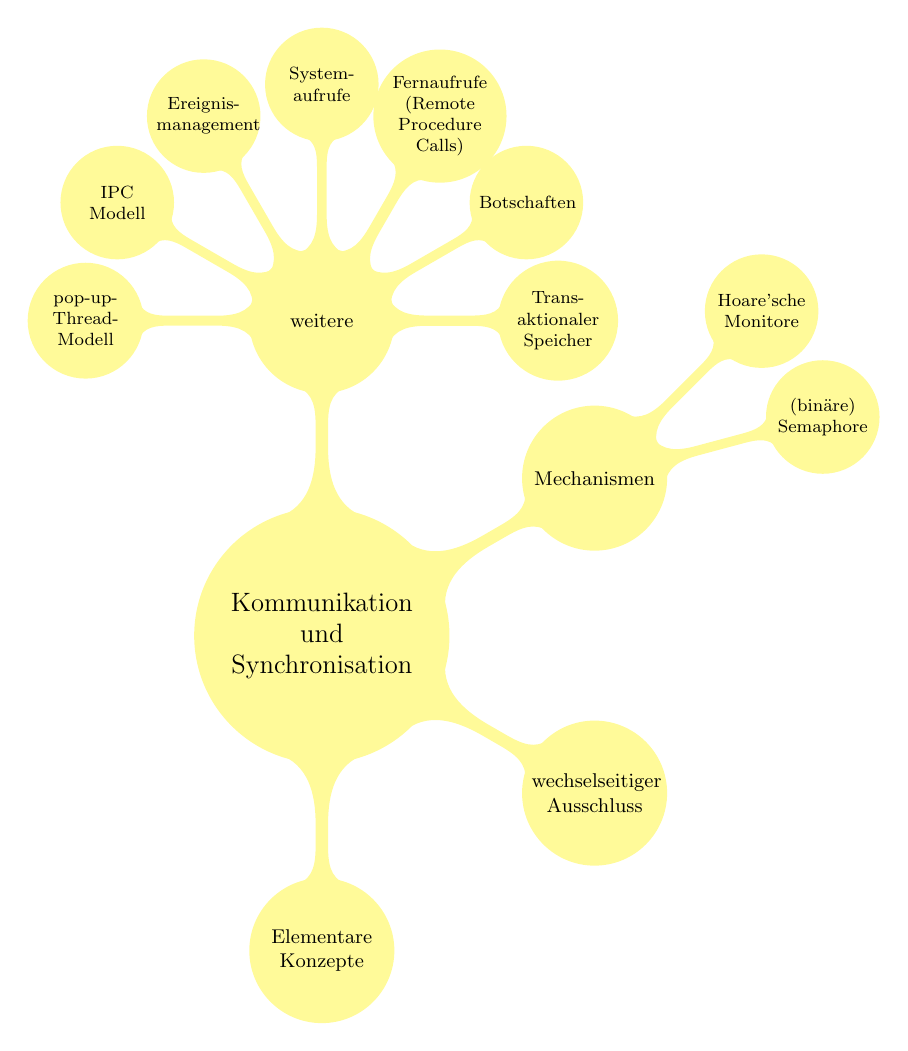
\begin{tikzpicture}[ mindmap, grow cyclic, every node/.style=concept, concept color=yellow!40,
    level 1/.append style={level distance=4cm},
    level 2/.append style={level distance=3cm, sibling angle=30},
    every node/.append style={scale=0.8}]
  \node{Kommunikation und \\Synchronisation}
  child { node {Elementare Konzepte}}
  child { node {wechselseitiger Ausschluss}}
  child { node {Mechanismen}
      child { node {(binäre) Semaphore}}
      child { node {Hoare'sche Monitore}}
    }
  child { node {weitere}
      child { node {Trans-aktionaler Speicher}}
      child { node {Botschaften}}
      child { node {Fernaufrufe (Remote Procedure Calls)}}
      child { node {System-aufrufe}}
      child { node {Ereignis-management}}
      child { node {IPC Modell}}
      child { node {pop-up-Thread-Modell}}
    };
\end{tikzpicture}

%%%%%%%%%%%%%%%%%%%%%%%%%%%%%%%%%%%%%% Speichermanagement
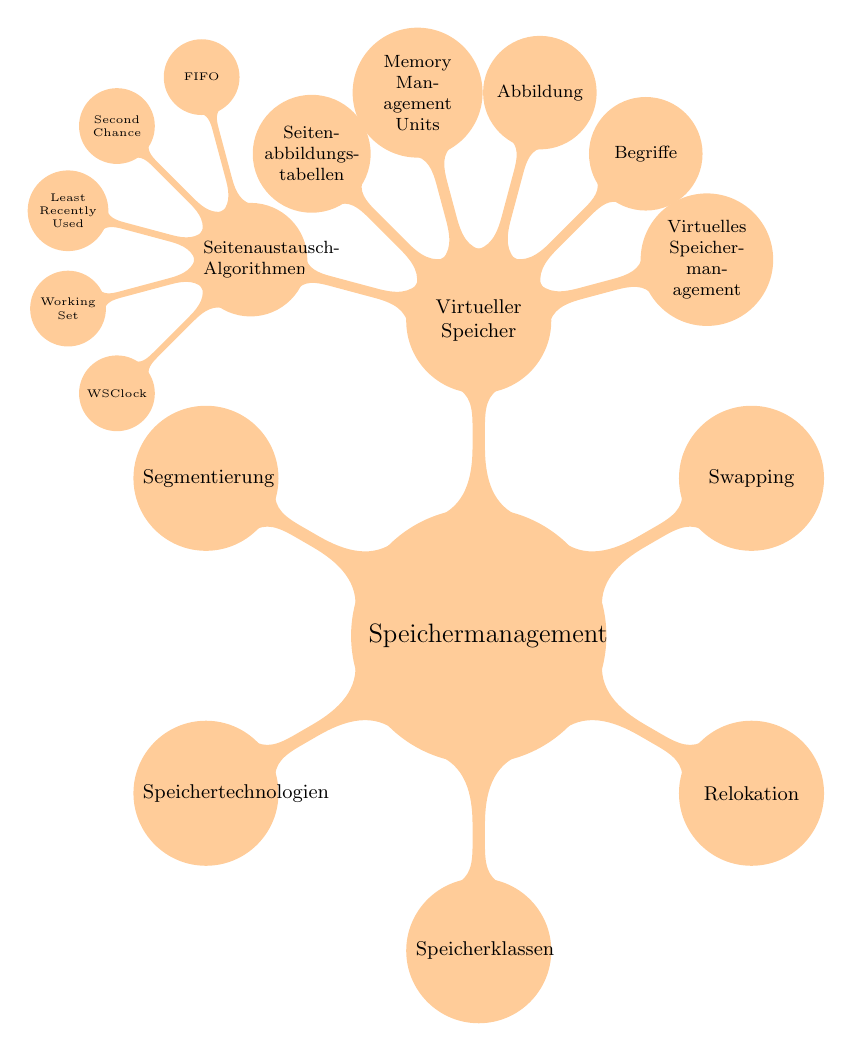
\begin{tikzpicture}[ mindmap, grow cyclic, every node/.style=concept, concept color=orange!40,
    level 1/.append style={level distance=4cm},
    level 2/.append style={level distance=3cm, sibling angle=30},
    every node/.append style={scale=0.8}]
  \node{Speichermanagement}
  child { node {Speichertechnologien }}
  child { node {Speicherklassen}}
  child { node {Relokation}}
  child { node {Swapping}}
  child { node {Virtueller Speicher}
      child { node {Virtuelles Speichermanagement}}
      child { node {Begriffe}}
      child { node {Abbildung}}
      child { node {Memory Management Units}}
      child { node {Seiten-abbildungs-tabellen}}
      child { node {Seitenaustausch-Algorithmen}
          child { node {FIFO}}
          child { node {Second Chance}}
          child { node {Least Recently Used}}
          child { node {Working Set}}
          child { node {WSClock}}
        }
    }
  child { node {Segmentierung}}
  ;
\end{tikzpicture}

%%%%%%%%%%%%%%%%%%%%%%%%%%%%%%%%%%%%%% Dateisystem
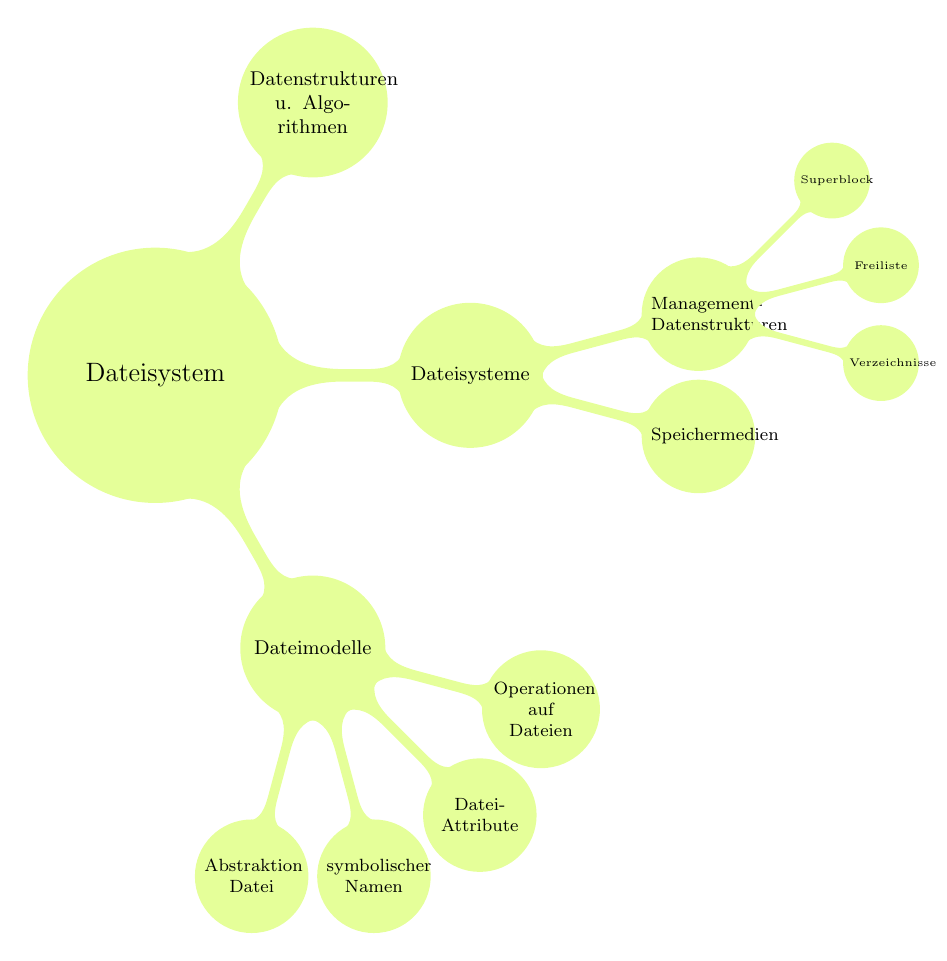
\begin{tikzpicture}[ mindmap, grow cyclic, every node/.style=concept, concept color=lime!40,
    level 1/.append style={level distance=4cm},
    level 2/.append style={level distance=3cm, sibling angle=30},
    every node/.append style={scale=0.8}]
  \node{Dateisystem}
  child { node {Dateimodelle}
      child { node {Abstraktion Datei}}
      child { node {symbolischer Namen}}
      child { node {Datei-Attribute}}
      child { node {Operationen auf Dateien}}
    }
  child { node {Dateisysteme}
      child { node {Speichermedien}}
      child { node {Management-Datenstrukturen}
          child { node {Verzeichnisse}}
          child { node {Freiliste}}
          child { node {Superblock}}
        }
    }
  child { node {Datenstrukturen u. Algorithmen}}
  ;
\end{tikzpicture}


\end{document}